\documentclass[10pt]{article}
\usepackage{a4wide}
\usepackage[english]{babel}
\usepackage{graphicx}
\usepackage{tabu}
\usepackage{textcomp}
\usepackage{fancyhdr}
\usepackage{lastpage}
\usepackage{titlesec}
\usepackage{lscape}
\usepackage{longtable}
\usepackage{color}
\usepackage{listings}
\usepackage{xkeyval}
\usepackage{hyperref}
\usepackage[utf8]{inputenc}
\usepackage{amsmath}
\usepackage{caption}
\usepackage{subcaption}
\usepackage{hhline}
\usepackage[titletoc,toc,title]{appendix}

\definecolor{mygreen}{rgb}{0,0.6,0}
\definecolor{mygray}{rgb}{0.5,0.5,0.5}
\definecolor{mymauve}{rgb}{0.58,0,0.82}

\lstset{ % Syntax highliughting for java
  backgroundcolor=\color{white},   % choose the background color; you must add \usepackage{color} or \usepackage{xcolor}
  basicstyle=\footnotesize,        % the size of the fonts that are used for the code
  breakatwhitespace=false,         % sets if automatic breaks should only happen at whitespace
  breaklines=true,                 % sets automatic line breaking
  captionpos=b,                    % sets the caption-position to bottom
  commentstyle=\color{mygreen},    % comment style
  deletekeywords={...},            % if you want to delete keywords from the given language
  escapeinside={\%*}{*)},          % if you want to add LaTeX within your code
  extendedchars=true,              % lets you use non-ASCII characters; for 8-bits encodings only, does not work with UTF-8
  frame=none,                      % adds a frame around the code
  keepspaces=true,                 % keeps spaces in text, useful for keeping indentation of code (possibly needs columns=flexible)
  keywordstyle=\color{blue},       % keyword style
  language=Octave,                 % the language of the code
  morekeywords={*,...},            % if you want to add more keywords to the set
  numbers=left,                    % where to put the line-numbers; possible values are (none, left, right)
  numbersep=5pt,                   % how far the line-numbers are from the code
  numberstyle=\tiny\color{mygray}, % the style that is used for the line-numbers
  rulecolor=\color{black},         % if not set, the frame-color may be changed on line-breaks within not-black text (e.g. comments (green here))
  showspaces=false,                % show spaces everywhere adding particular underscores; it overrides 'showstringspaces'
  showstringspaces=false,          % underline spaces within strings only
  showtabs=false,                  % show tabs within strings adding particular underscores
  stepnumber=5,                    % the step between two line-numbers. If it's 1, each line will be numbered
  stringstyle=\color{mymauve},     % string literal style
  tabsize=4,                       % sets default tabsize to 2 spaces
  title=\lstname                   % show the filename of files included with \lstinputlisting; also try caption instead of title
}
%%%%%%
%% Variables for version and release status
%% useage: \version
%%%%%%
\newcommand\module{CS36110}
\newcommand\assignmentTitle{Assignment 2 - MNIST Dataset}
\newcommand\authorText{Nicholas Dart}
\newcommand\authorUsername{nid21}
\newcommand\studentID{130057750}
\newcommand\assesser{Dr Christine Zarges}

%%%%%%
%% Alias
%%%%%%
%\newcommand{\sectionbreak}{\clearpage}    %% Allways start a section on a new page
\newcommand\wordcount{
  \input{|"texcount \jobname.tex | grep 'Words in text' | awk '{print $4}'"}\unskip
}

\title{ \huge \module~Assignment \\ \Large \assignmentTitle}
\author{
  \vspace{100pt}
  \begin{tabular}{ r || l }
    Author          & \authorText~(\authorUsername)\\
                    & \studentID \\
    Date Published  & \today \\
                    & \\
    Assessed By     & \assesser \\
    Department      & Computer Science \\
    Address         & Aberystwyth University \\
                    & Penglais Campas \\
                    & Ceredigion \\
                    & SY23 3DB \\
  \end{tabular} \\
  Copyright \textcopyright~Aberystwyth University 2016
  %get rid of the date on the titlepage
  \date{}
}

\pagestyle{fancy}
\fancyhf{}
\lhead{\module~Assignment}
\rhead{\authorText~-~\studentID}
\rfoot{Page \thepage \hspace{1pt} of \pageref{LastPage}}
\lfoot{Aberystwyth University - Computer Science}

\begin{document}
  \setcounter{page}{1}

  \maketitle
  \thispagestyle{empty}
  \clearpage

  \tableofcontents
  \clearpage

  \section{Introduction}
    This assignment was undertaken using WEKA 3.6.10, using the provided data sets. This report length is \wordcount, not including headers, references, appendix or title page.\\

    I partially worked with Xander Barnes (acb12) on the first part of the second task in this assignment. We worked together to produce the initial run of epochs for Multilayer Perceptrons shown in table \ref{table:mlpEpochTest}.

    I ran the data sets on a number of machines;

    \begin{enumerate}
      \item i7-3770 CPU @ 3.40GHz Desktop (For tasks in section \ref{sec:1} and \ref{sec:2B})
      \item Microsoft Azure GS3 \cite{azureGSseries} Instance (For tasks in subsection \ref{sec:2A})
    \end{enumerate}

  \section{Task 1 - Feature Selection}
    \label{sec:1}

    The following steps are carried out with the \texttt{MNIST\_784-train60000} data sets, using the \texttt{MNIST\_784-test10000} set for testing.\\

    \subsection{Preprocessing}
      \label{sec:1A}
      My initial thought about preprocessing the input data is that large numbers of the features that make up a digit image are likely to be composed of entirely white (value of 0) or black (value of 255), especially towards the corners and the left and right edges as the images were centred within the 28x28 pixel image \cite{mnistDatabase}. These features can easily be identified from within WEKA (see figure \ref{fig:wekaUselessFeature}), and could be removed as they provide no useful information that will aid in classifying the digit image. \\

      Standard deviation and mean vary among the the different features (figure \ref{fig:wekaUselessFeature} and figure \ref{fig:wekaHighStdDev}). Features with low standard deviations are likely to have values clustered very close together, and so provide less useful information for classifying.

      Ideal features for classification will be ones that contain a high value for one or more classes, and a low value for others. These key features could then be used together to make a prediction of which class the instance belongs to. In addition it could be useful to combine lower resolution image features along with higher ones (for example features of an 14x14 and 8x8, 4x4, etc) to provide a more information to the classifier.

      I used the \textbf{RemoveUseless} filter in the preprocessing tab. This filter removes any features whose values do not vary at all (therefore provided no classification value), as well as any features whose variance percentage is greater than a definable value. Doing this with a variance percentage of 100 removes 67 attributes, as expected they were located around the edge of the image, as showing in figure \ref{fig:visualisedRemoveUnused}. This corresponds to what I would expect, however I also expect that other features that lie further in from the edge of the image to have similarly useless images with only one or two values that differ from the mean.

      Thinking along these lines I also removed all features whose mean is less than 1 as these features were likely to contain a large proportion of white. I expected the trend to continue in that features nearer the outsides of the image to be more likely to be removed. I chose a threshold of 1 arbitrarily, but believe that it will likely only filter out attributes who have all white values except one or two. The results as shown in figure \ref{fig:visualisedRemoveMean} show that my guess was correct.

      \begin{figure}
        \centering

        \begin{subfigure}[t]{.5\textwidth}
          \centering
          \caption{An attribute with a very high standard deviation}
          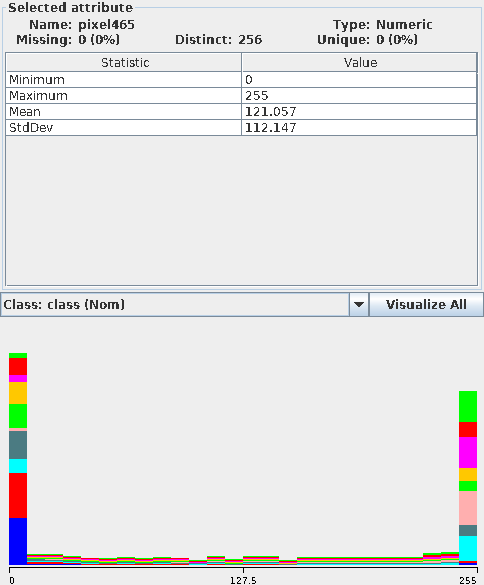
\includegraphics[width=0.9\linewidth]{weka-high-stdDev.png}
          \label{fig:wekaHighStdDev}
        \end{subfigure}%These comments are very important ??  https://tex.stackexchange.com/questions/37581/latex-figures-side-by-side
        \begin{subfigure}[t]{.5\textwidth}
          \centering
          \caption{A ``useless'' attribute with all instances of value 0}
          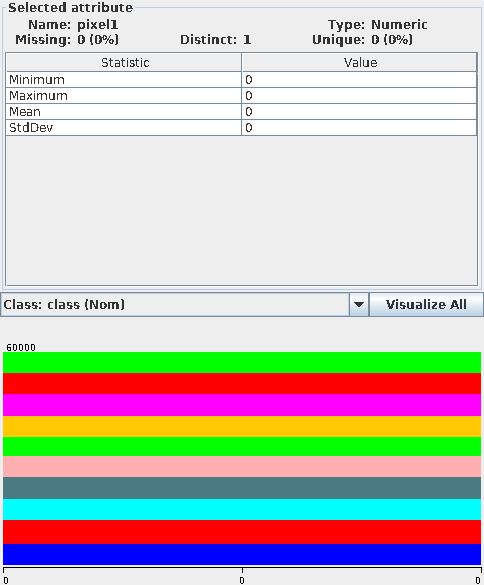
\includegraphics[width=0.9\linewidth]{weka-useless-feature.png}
          \label{fig:wekaUselessFeature}
        \end{subfigure}

        \caption{Weka attribute details panels for two attribute}
        \label{fig:wekaFeature}
      \end{figure}

      \begin{figure}
        \centering

        \begin{subfigure}[t]{.5\textwidth}
          \centering
            \caption{Removed ``useless'' attributes}
            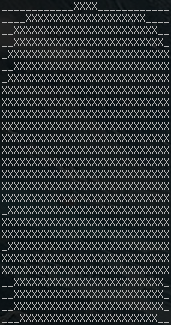
\includegraphics[scale=1]{visualisedRemoveUnused.png}
          \label{fig:visualisedRemoveUnused}
        \end{subfigure}%
        \begin{subfigure}[t]{.5\textwidth}
          \centering
            \caption{Removed with mean\textless1}
            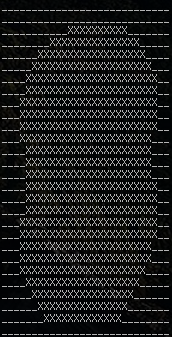
\includegraphics[scale=1]{visualisedMeanRemoval.png}
          \label{fig:visualisedRemoveMean}
        \end{subfigure}

        \caption{Visualisation of removed attributes.\\\textbf{\_} are removed attribute positions,\\\textbf{X} are kept attribute positions}
        \label{fig:visualisedRemove}
      \end{figure}

    \subsection{Training}
      Training J48 and Naïve Bayse on the \texttt{mnist784-train6000.arff} (and using the \texttt{mnist784-test10000.arff} set for test) gave results in table \ref{table:task1initialTrainResults}.

      Both J48 and Bayse produced reasonably accurate classifiers based on True Positive (TP) and False Positive (FP) rates, and both classifiers were very quick to run on the largest training and test sets. In this instance Naïve Bayse, which is considered the benchmark for machine learning classifiers, was outperformed by J48, although Bayse was significantly faster to run. 

      J48 produced a tree with 2228 leaves without pruning, and 1130 leaves with pruning. Interestingly J48 (pruned and unpruned) determined that \textbf{pixel101} was the most important pixel for classification, but as might be expected partitioned the values on \texttt{\textless=0} and \texttt{\textgreater0}, thus effectively checking if it is fully white or not.

      Looking back at Bayse, it had a tendency to misclassifying as class eight or nine more than any other class. eights were frequently misclassified as 2, 3 or 5 and nines as 4, 7 or 8, likely as a result of their similarity, but also probably as a result of the numbers being written askew.

      \begin{table}
        \centering
        \begin{tabular}{ | r | l | l | l | l | }
          \hline
          Classifier   & Time (s) & TP Rate & FP Rate & Precision \\ \hhline{|=|=|=|=|=|}
          Naïve Bayse  & 4.31     & 0.697   & 0.033   & 0.746     \\ \hline
          J48 unpruned & 153.55   & 0.893   & 0.012   & 0.893     \\ \hline
          J48 pruned   & 91.45    & 0.879   & 0.013   & 0.879     \\ \hline
        \end{tabular}
        \caption{Classification results on unmodified mnist784 data}
        \label{table:task1initialTrainResults}
      \end{table}

    \subsection{Retraining with cleaned Dataset}
      Using the data set I constructed from section \ref{sec:1A}, I managed to achieve reduced model build times across the board as shown in table \ref{table:task1RetrainResults}. Naïve Bayse also performed better on the reduced data sets as well, achieving a higher True Positive classification and lower Positive, when compared with the initial training.

      After cleaning, J48 produced a tree with 2228 leaves (unpruned) and and 1146 leaves (pruned). For both the pruned and unpruned trees when compared with their original counterparts, the subtree of \texttt{pixel101 \textgreater 0} was identical to that in the initial training. 

      \begin{table}
        \centering
        \begin{tabular}{ | r | l | l | l | l |}
          \hline
          Classifier   & Time (s)  & TP Rate & FP Rate & Precision \\ \hhline{|=|=|=|=|=|}
          Naïve Bayse  & 2.92      & 0.735   & 0.029   & 0.765     \\ \hline
          J48 unpruned & 104.78    & 0.89    & 0.012   & 0.889     \\ \hline
          J48 pruned   & 61.13     & 0.874   & 0.014   & 0.874     \\ \hline
        \end{tabular}
        \caption{Classification results on modified mnist784 data}
        \label{table:task1RetrainResults}
      \end{table}

  \section{Task 2 - Multilayer Perceptrons}
    \label{sec:2}

    I chose to use Multilayer Perceptrons as I understand their concept better than Support Vector Machines. I have also used Google's Tensorflow in the past, so wanted to further explore the field of Artificial Neural Networks.\\

    Multilayer Perceptrons in WEKA have a number of options that can be changed. They include;

    \begin{itemize}
      \item ``Learning Rate'' is adjustment to neuron weights after each epoch.
      \item ``Decay'' is the multiplier to apply to the learning rate after each epoch \cite{wekaGitMirrorDecay}.
      \item ``Hidden Layers'' is a description of the number of hidden layers, and then number of units in the layer (Some wildcards exist here to represent the number of neurons in relation to feature or class count).
      \item ``Momentum'' is a feature that allows for escaping of local minimum when going down gradient descent.
      \item ``Training Time'' is the number of epochs or learning iterations to go through.
      \item ``Validation Set Size'' is the amount of the validation or test set to use to determine when the training has reached it's end or best.
      \item ``Validation Threshold'' is the number of iterations after which if the training has been getting worse results against the \texttt{Validation Set} to be stopped.
    \end{itemize}
    
    \subsection{Training}
      \label{sec:2A}
      
      We (Xander Barnes and I) tested the default options on the \texttt{mnist576-train-1500} data set, and then lowered the number of epochs to try reduce the amount of time taken to learn. The results are shown in table \ref{table:mlpEpochTest}. Doing this I realised to my surprise that even an ANN with only one iteration of back propagation could achieve reasonable accuracy in a very short amount of time.

      It is also clear from the time taken increases almost linearly with number of epochs, however for this increase in time there is only very small increases in True Positive (TP) identification rates, and conversely small rates in decrease of False Positive (FP) rates, and for the default settings, there were no increases in performance or precision after somewhere between 5 and 25 iterations.\\

      Taking this further I decided to try relatively few neurons with only one iteration of back propagation to see how well a MLP could achieve, and where it would break down, the results are shown in table \ref{table:mlpHiddenLayerTest}. Graphing the results in figure \ref{fig:mlp10HiddenUnits}, we can see the clear drop off in the rate of improvement as the number of neurons in the hidden layer increases.

      I was unable to explain why there was a decrease in performance when moving from 6 to 7 neurons, however was able to reproduce the results consistently.\\

      I further decided to expand on this by increasing the number of learning iterations to two and trying 1 through 15 units in then hiden layer again to see how learning iterations changes the result. The results for this test are graphed in figure \ref{fig:mlp10HiddenUnits2Iterations}.

      It is interesting to see that and to achieve 75\% classification accuracy, only 10 neurons are needed for a single learning iteration, and for two iterations that is lowered to seven. \\

      \begin{table}
        \centering
        \begin{tabular}{ | r | l | l | l | l | }
          \hline
          Epochs & Time (s) & TP    & FP    & Precision \\ \hhline{|=|=|=|=|=|}
          500    & 1874.12  & 0.978 & 0.002 & 0.978     \\ \hline
          250    & 993.5    & 0.979 & 0.002 & 0.979     \\ \hline
          50     & 210.2    & 0.977 & 0.003 & 0.977     \\ \hline
          25     & 104.88   & 0.977 & 0.003 & 0.977     \\ \hline
          5      & 15.03    & 0.968 & 0.004 & 0.968     \\ \hline
          2      & 6.59     & 0.949 & 0.006 & 0.952     \\ \hline
          1      & 3.67     & 0.943 & 0.006 & 0.945     \\ \hline
        \end{tabular}

        \caption{MLP with varied number of epochs}
        \label{table:mlpEpochTest}
      \end{table}

      \begin{table}
        \centering
        \begin{tabular}{ | r | l | l | l | }
          \hline
          Units & TP & FP & Precision \\ \hhline{|=|=|=|=|}
          15 & 0.852 & 0.017 & 0.867  \\ \hline
          14 & 0.852 & 0.017 & 0.867  \\ \hline
          13 & 0.83  & 0.018 & 0.773  \\ \hline
          12 & 0.832 & 0.018 & 0.766  \\ \hline
          11 & 0.809 & 0.02  & 0.744  \\ \hline
          10 & 0.766 & 0.026 & 0.699  \\ \hline
          9 & 0.722  & 0.032 & 0.606  \\ \hline
          8 & 0.502  & 0.055 & 0.476  \\ \hline
          7 & 0.249  & 0.078 & 0.093  \\ \hline
          6 & 0.474  & 0.056 & 0.358  \\ \hline
          5 & 0.264  & 0.084 & 0.126  \\ \hline
          4 & 0.09   & 0.09  & 0.008  \\ \hline
          3 & 0.09   & 0.09  & 0.008  \\ \hline
          2 & 0.092  & 0.092 & 0.008  \\ \hline
          1 & 0.092  & 0.092 & 0.008  \\ \hline
        \end{tabular}

        \caption{MLP with varied number of hiden units in one layer}
        \label{table:mlpHiddenLayerTest}
      \end{table}

      \begin{figure}
        \centering
        \captionsetup{justification=centering}
          \caption{1 to 15 Neurons in one hidden layer. Graph of data from table \ref{table:mlpHiddenLayerTest}}
          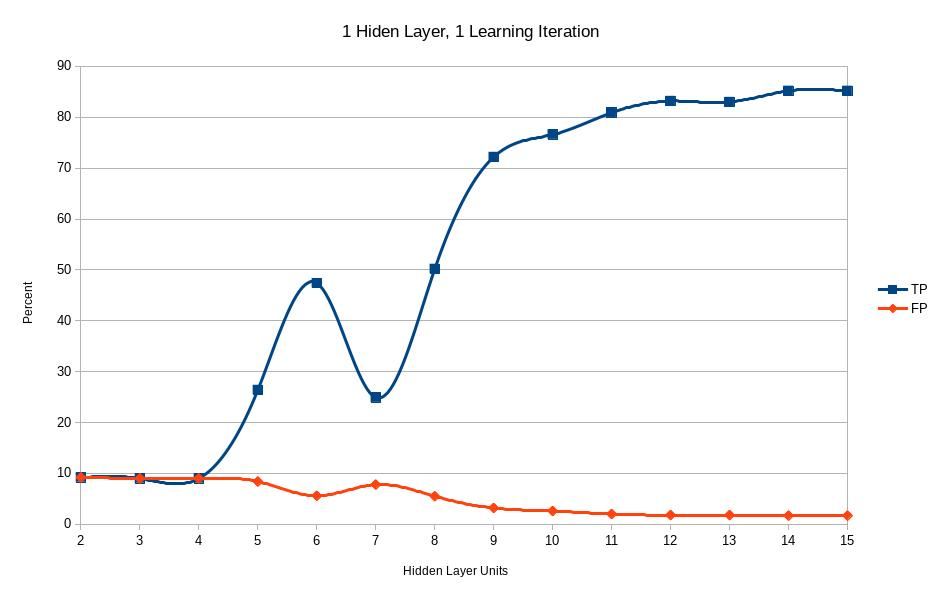
\includegraphics[width=\textwidth]{ann-10-units-1-iteration.jpg}
        \label{fig:mlp10HiddenUnits}
      \end{figure}

      \begin{figure}
        \centering
        \captionsetup{justification=centering}
          \caption{1 to 15 Neurons in one hidden layer with 2 learning iterations}
          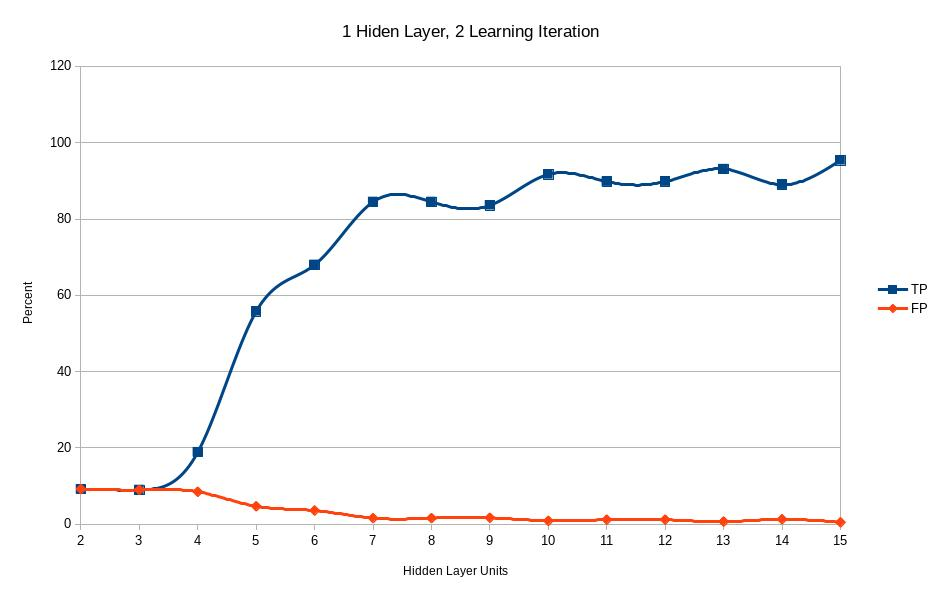
\includegraphics[width=\textwidth]{ann-10-units-2-iteration.jpg}
        \label{fig:mlp10HiddenUnits2Iterations}
      \end{figure}

    \subsection{Comparison}
      \label{sec:2B}
      Using the data I collected from part 2A (Section \ref{sec:2A}), I decided to use the default settings for Multilayer Perceptron, but changed the number of neurons in the hidden layer to 50 and the number of epochs to 5. I also ran J48 with pruning enabled and disabled. The results of these tests are shown in table \ref{table:mlpComparison}.

      My Multilayer Perceptron had a comparable classification precision to Bayse for the reduced \texttt{576} data set of \texttt{0.964} and \texttt{0.937}, however Bayse was significantly quicker to train the model. J48 was similarly timed for both sized data sets and comparable to MLP for the \texttt{576} feature set.

      Overall Multilayer Perceptrons with 50 neurons in a single hidden layer and 5 training iterations achieved about on par with Bayse and J48 for both data sets, however Bayse significantly outperformed in training time, due to it's simple nature. J48 performed better on the larger data set when no \texttt{reduced error pruning} was performed, but better on the smaller data set with pruning, although enabling pruning achieved a reduction in learning time by almost half.

      From the data, Bayse seems like the best option to choose when classifying the \texttt{MNIST} data set as it is far quicker than the rest, but achieves comparable results. Bayse also has the inherent ability to be quickly retrained in the future which would make it a better choice for applications where the classifier can be provided with feedback about it's output. 

      \begin{table}
        \centering
        \begin{tabular}{ | r | l | l | l | l | l | }
          \hline
                       & Features & Time (s) & TP    & FP    & Precision \\ \hhline{|=|=|=|=|=|=|}
          MLP          & 576      & 188.65   & 0.963 & 0.004 & 0.964     \\ \hline
          MLP          & 784      & 323.26   & 0.884 & 0.012 & 0.889     \\ \hhline{|=|=|=|=|=|=|}
          Bayse        & 576      & 5.64     & 0.935 & 0.007 & 0.937     \\ \hline
          Bayse        & 784      & 6.67     & 0.697 & 0.033 & 0.746     \\ \hhline{|=|=|=|=|=|=|}
          J48 Unpruned & 576      & 208.12   & 0.893 & 0.012 & 0.893     \\ \hline
          J48 Unpruned & 784      & 214.73   & 0.949 & 0.006 & 0.949     \\ \hhline{|=|=|=|=|=|=|}
          J48 Pruned   & 576      & 123.23   & 0.942 & 0.006 & 0.942     \\ \hline
          J48 Pruned   & 784      & 122.71   & 0.879 & 0.013 & 0.879     \\ \hline
        \end{tabular}

        \caption{MLP compared to Bayse and J48 for the different feature sizes}
        \label{table:mlpComparison}
      \end{table}

  \begin{thebibliography}{9}

    \bibitem{mnistDatabase}
      MNIST database of hand written digits (Accessed 11/12/16)\\
      \url{http://yann.lecun.com/exdb/mnist/}

    % \bibitem{} 
    %   Willamette University. Genevieve B. Orr. CS449 - Neural Networks cource (Accessed 11/12/16)\\
    %   \url{https://www.willamette.edu/~gorr/classes/cs449/momrate.html}

    \bibitem{azureGSseries}
      Microsoft Azure GS series Cloud Computing Instances (Accessed 14/12/16)\\
      \url{https://azure.microsoft.com/en-gb/blog/azure-has-the-most-powerful-vms-in-the-public-cloud/}

    \bibitem{wekaGitMirrorDecay}
      Github Mirror of Weka Source
      \url{https://github.com/bnjmn/weka/blob/cfb4b4e4fabca3b54a5b7defd54b8e944801864f/src/main/java/weka/classifiers/functions/MultilayerPerceptron.java#L1955}
  \end{thebibliography}

\end{document}
